\documentclass[12pt]{report}

\usepackage[utf8]{inputenc} % utf8 encoding
\usepackage[T2A]{fontenc}
\usepackage[english,russian]{babel}

\usepackage[
	autolang=hyphen,
	language=auto,
	autolang=other,
	backend=biber,
	style=gost-numeric
]{biblatex}
\addbibresource{reviews.bib}

\DeclareSourcemap{
	\maps[datatype=bibtex, overwrite]{
		\map{
			\step[fieldset=langid, fieldvalue=english]
			\step[fieldset=doi, null]
			\step[fieldset=issn, null]
			\step[fieldset=isbn, null]
			\step[fieldset=url, null]
			\step[fieldsource=language, fieldset=langid, origfieldval]
		}
	}
}

\usepackage{graphicx}
\graphicspath{{../../images/}}

\usepackage{amsmath,amsfonts,amsthm,amssymb} % nice math symbols
\usepackage{hyperref}
\hypersetup{%
	pdfencoding=auto,
	pdfauthor={Александр Панов},
	pdftitle={Обзоры}
}

\title{Обзоры к отчетам}
\author{А.\,И.~Панов}

\begin{document}
	\chapter{Концептуальные модели в нейрофизиологии}
	\section{Типы обучения и подсистемы мозга}
	
	Основная задача реинжениринга мозга - построить глобальную непротиворечивую модель мозга, основываясь на имеющихся в литературе данных и теориях \cite{Shumsky2015b}. Основными подсистемами мозга, осуществляющими обучение и контроль поведения, по имеющимся представлениям являются кора головного мозга (в частности, новая кора(неокортекс) и старая кора (аллокортекс), включающая гиппокамп), тесно связанная с таламусом, базальные ганглии и мозжечок. Каждая из этих подсистем мозга, предположительно, реализует свой тип обучения: обучение без учителя (таламо-кортикальная система), обучение с подкреплением (базальные ганглии) и обучение с учителем (мозжечок) \cite{Doya2000a} (рис. \ref{fig:doya_schema}).
	\begin{figure}[h]
		\centering
		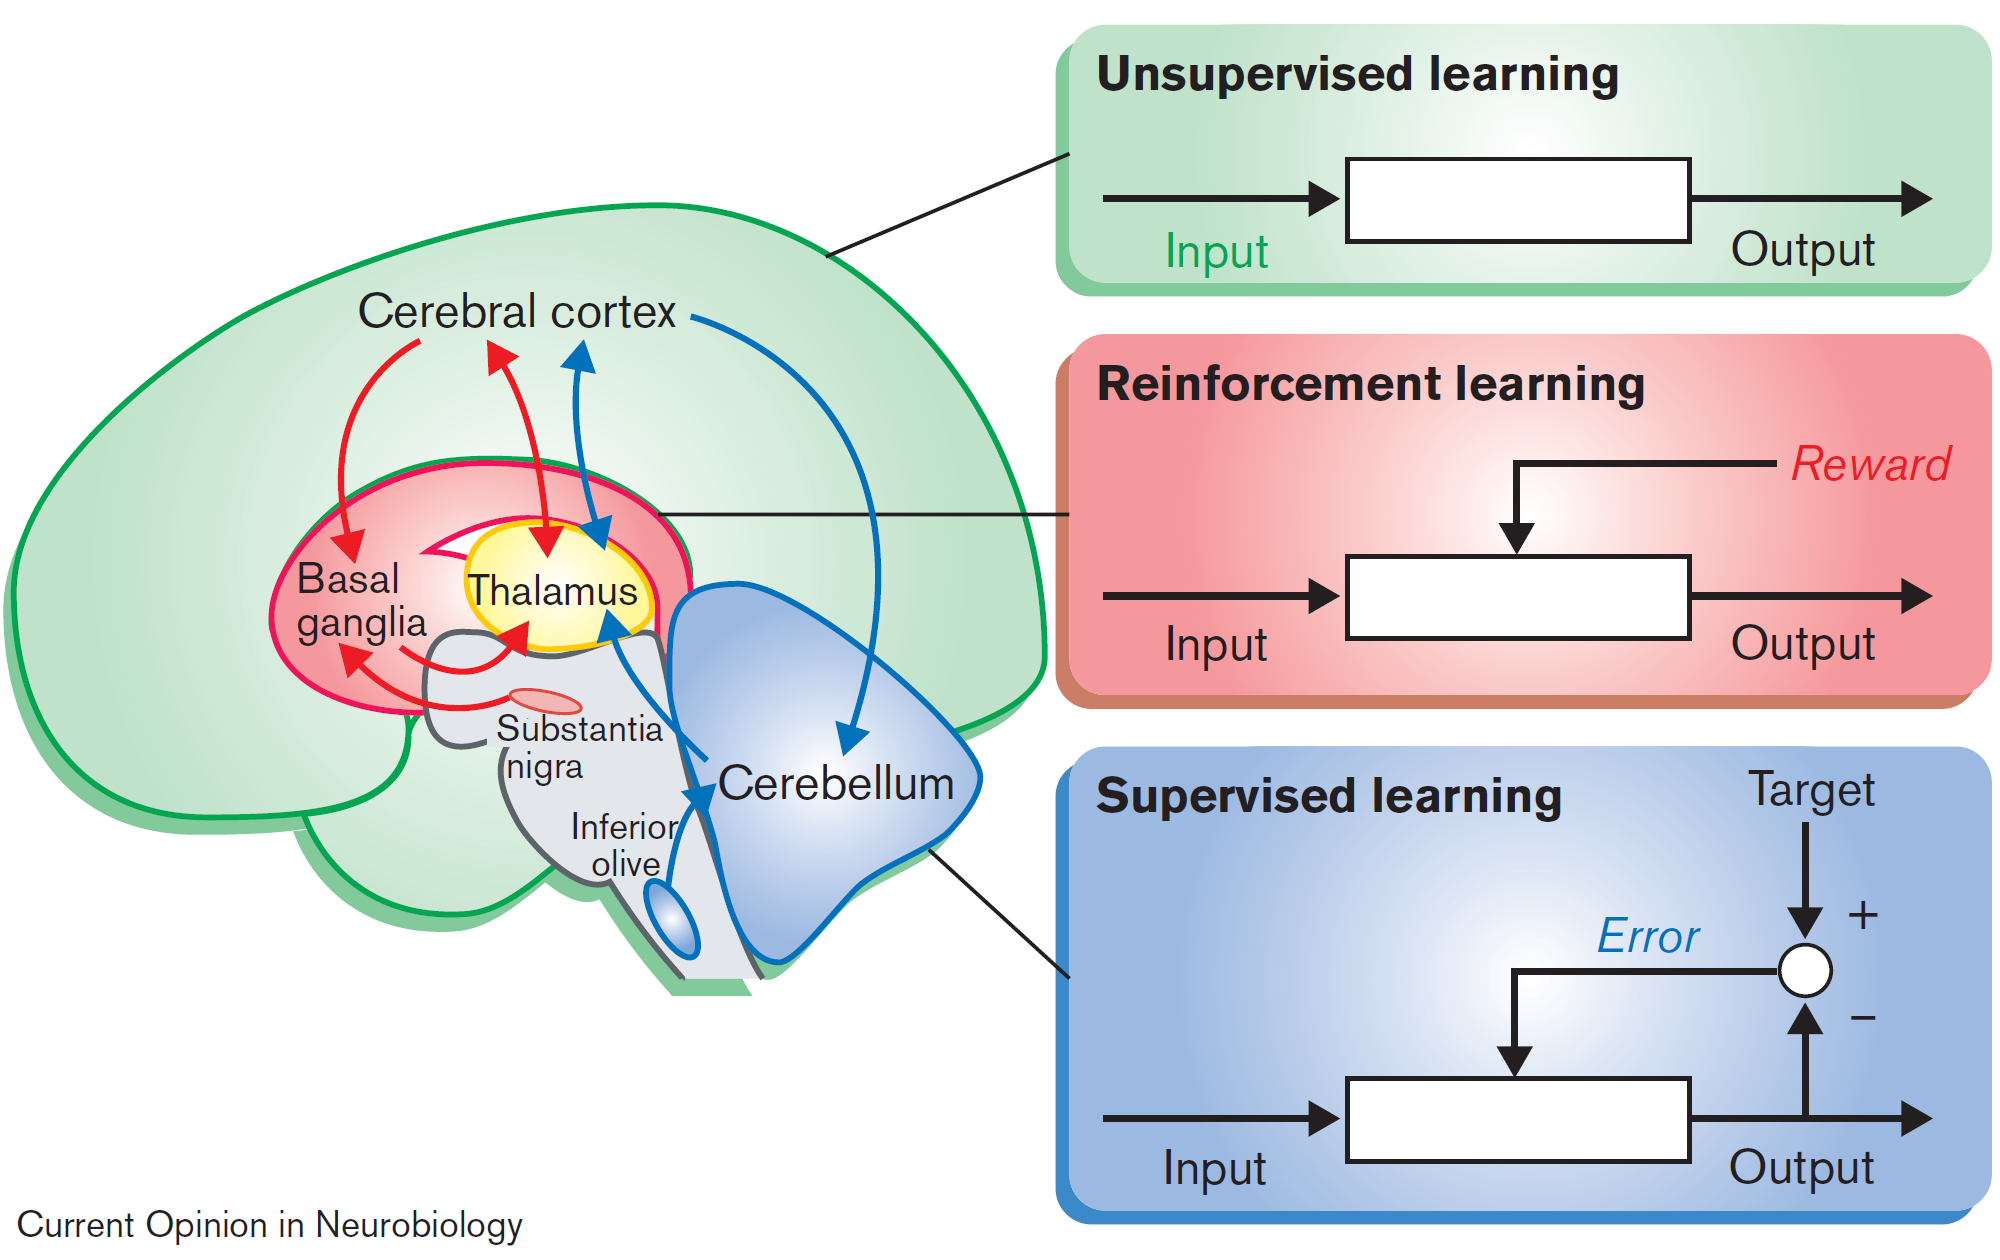
\includegraphics[width=0.7\textwidth]{misc/phisio/doya_schema}
		\caption{Различные типа обучения, реализуемые мозжечком, базальными ганглиями и корой головного мозга (взято из \cite{Doya2000a})}.
		\label{fig:doya_schema}		
	\end{figure}

	Перечисленный выше подсистемы мозга принимают совместное участие в различных контурах, управляющих нашим поведением \cite{Shumsky2015b} (рис. \ref{fig:control_loops} и \ref{fig:control}). Таламо-кортикальная система выявляет временные и пространственные паттерны в поступающих через органы чувств сигналах внешней среды. Моторная часть коры совместно с базальными ганглиями и таламусом вырабатывает ответную реакцию организма, соответствующую предыдущему опыту действования и текущей ситуации. Наконец, мозжечок выполняет многократно повторенные ранее действия, автоматизированные и практически не встречающие препятствий в своей реализации.
	
	\begin{figure}
		\centering
		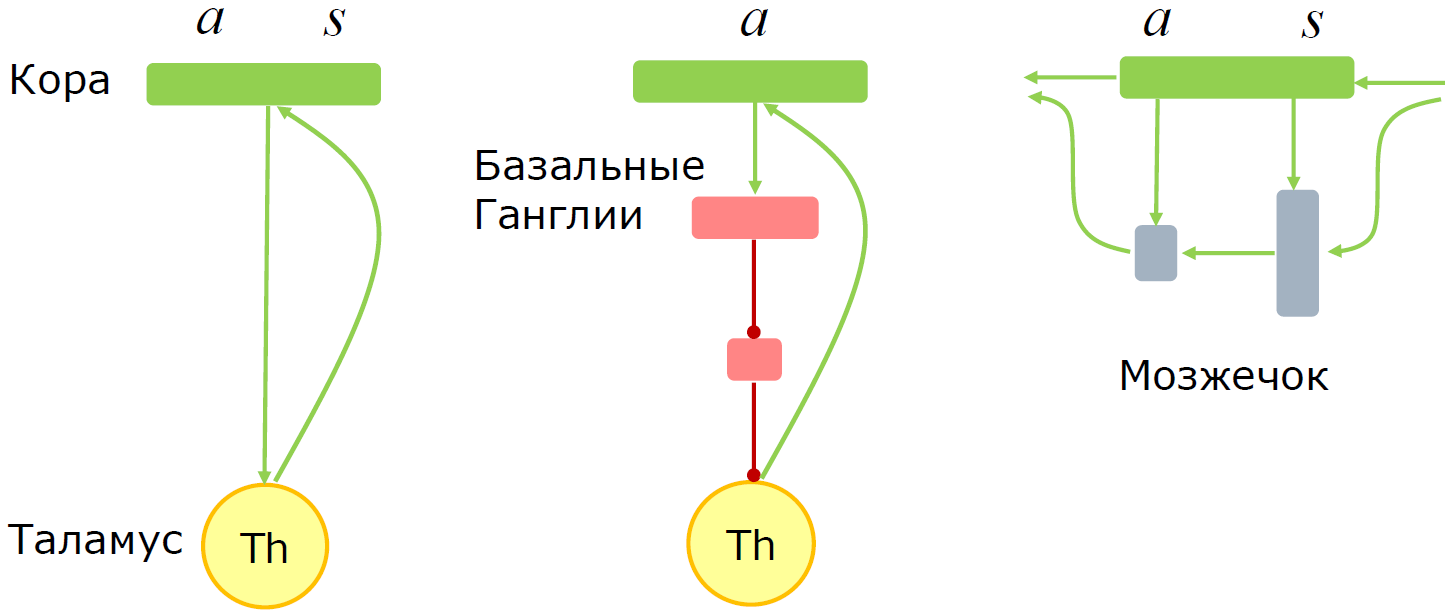
\includegraphics[width=0.7\textwidth]{misc/phisio/shumsky_loops}
		\caption{Управляющие контуры в головном мозге, $a,s$ - участки коры, ответственны за распознавание ситуации и выработку моторного действия, соответственно (взято из \cite{Shumsky2015b})}
		\label{fig:control_loops}		
	\end{figure}

	Кора головного мозга делится на преобладающую у человека новую кору (неокортекс), состоящий из 5 слоев нервных клеток, и филогенетически более раннюю старую кору (палеокортекс и архитокортекс), состоящую из 3--5 слоев. Все участки коры имеют тесные связи с таламусом \cite{Izhikevich2008} (рис. \ref{fig:cotr_talam}), что и объясняет их объединение в таламо-кортикальную систему. Пирамидальные клетки и их дендриты из второго и третьего слоя (L2/3) принимают сигналы от других участков коры (кортико-кортикальные связи). Нейроны четвертого слоя (L4) интегрируют информацию, получаемую от таламуса и других подкорковых структур, с информацией от разных участков коры. Пятый слой (L5) собирает полученную информацию и передает ее в подкорковые структуры (базальные ганглии) и через шестой слой - в таламус и другие участки коры. При этом нейроны L5 служат кодирующим слоем рекуррентной сети, текущее состояние которой поступает из слоя L2/3 и в слое L4 дополняется сжатым предыдущим состоянием (предисторией) от таламуса, который в свою очередь получил его с некоторой временной задержкой из выходных слоев L5 и L6.
	
	\begin{figure}
		\centering
		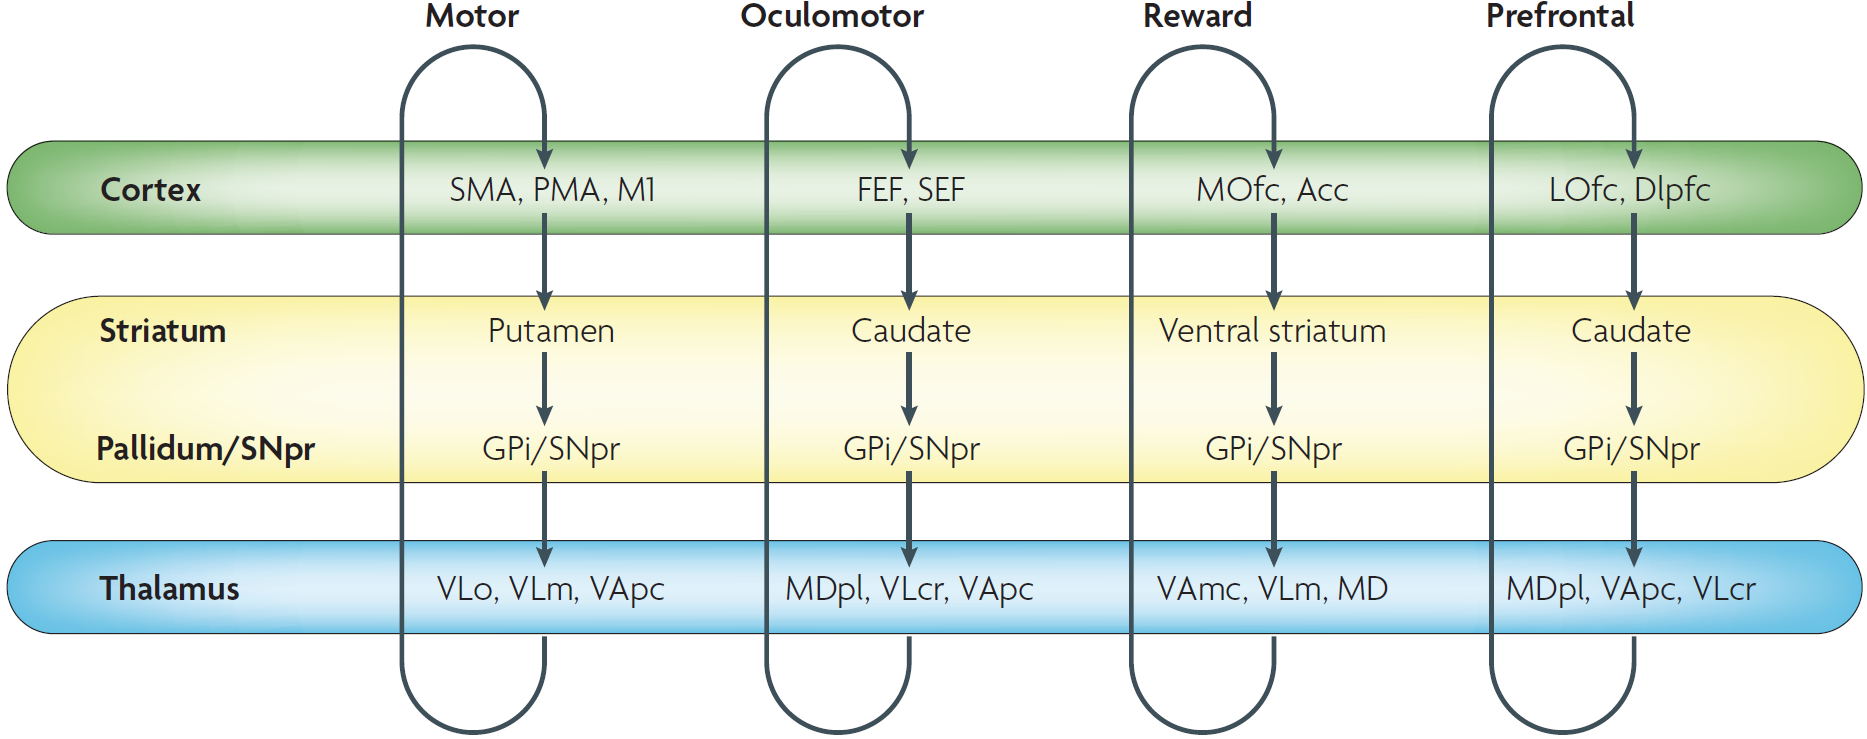
\includegraphics[width=0.8\textwidth]{misc/phisio/control_loops}
		\caption{Параллельные управляющие циклы, проходящие через кору, базальные ганглии и таламус (взято из \cite{Kringelbach2007})}
		\label{fig:control}		
	\end{figure}

	\begin{figure}
		\centering
		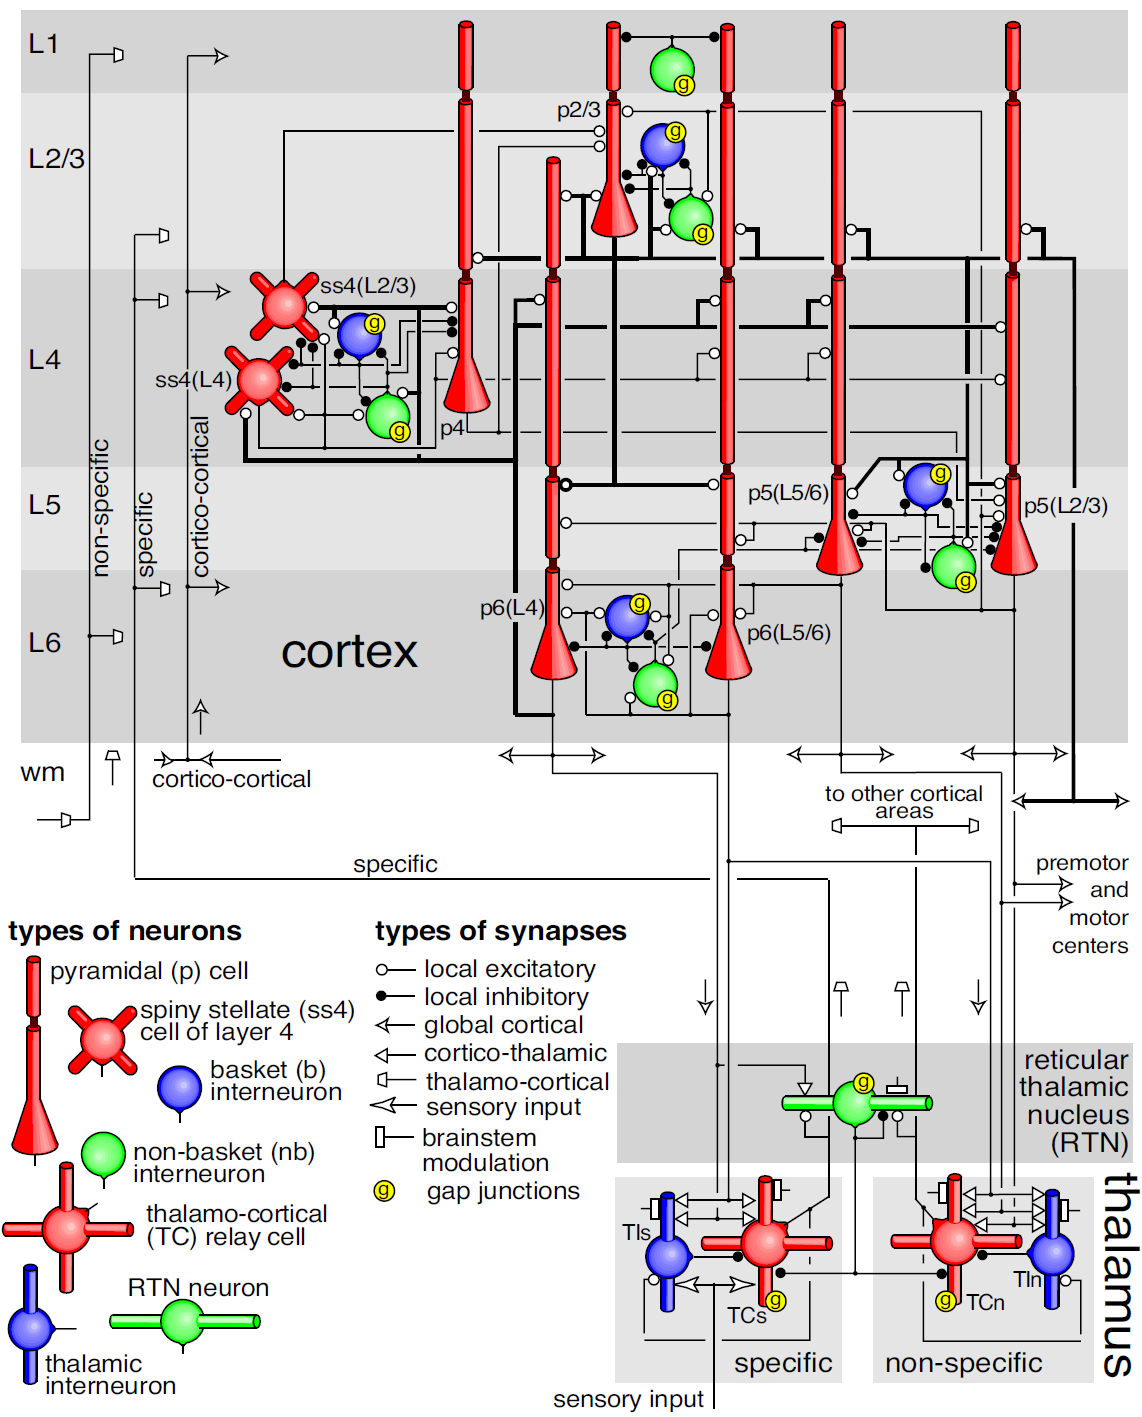
\includegraphics[width=0.7\textwidth]{misc/phisio/cort-talam_loop}
		\caption{Диаграмма нейронных цепей продольной структуры коры и таламических ядер (взято из \cite{Izhikevich2008})}
		\label{fig:cotr_talam}		
	\end{figure}

	В целом кора кодирует наблюдаемую ситуацию как устойчивое сочетание значений признаков с предсказанием того, что должно последовать за этой ситуацией. Значения признаков являются результатом возбуждения некоторой колонки (диаметр 300-500 мкм, количество нейронов $10^4$) в рамках группы локально конкурирующих колонок (гиперколонки - диаметром 2-3 мм). Всего в коре получается около $10^5$ гиперколонок, т.е. кодируется до миллиона различных признаков. В отличие от новой коры, участки старой коры, в частности гиппокамп, могут кодировать только ассоциативные связи, а не типовые паттерны, подобно разреженной сети Хопфилда. Так как у человека входами гиппокампа являются выходы коры, то гиппокамп хранит в себе эпизодическую категориальную память, ограниченной емкости, которая затем в результаты проигрывания во время сна, консолидируется корой (рис. \ref{fig:hippocamp}).
	
	Все участки коры образуют две тесно связанные друг с другом параллельные иерархии - сенсорную и моторную, в которых активация распространяется в противоположных направлениях. Предполагается, что вершиной сенсорной иерархии является гиппокамп, а корнем моторной - поясная извилина коры. В свою очередь гиппокамп и поясная извилина входят в состав лимбической подсистемы мозга, которая как раз и ответственная за выработку поведения с учетом эмоционально-потребностной сферы.

	\begin{figure}
		\centering
		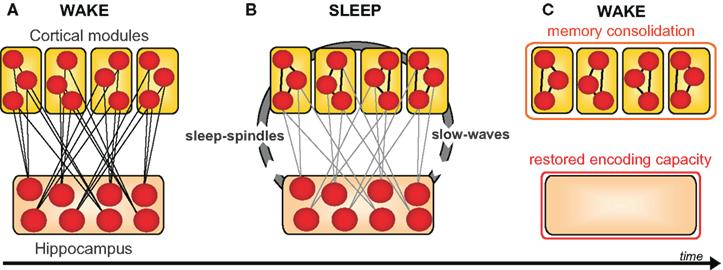
\includegraphics[width=0.8\textwidth]{misc/phisio/hippocamp_sleep}
		\caption{Консолидация эпизодической памяти в кору головного мозга из гиппокампа (взято из \cite{Saletin2012})}
		\label{fig:hippocamp}		
	\end{figure}	

	
	Моторная иерархия головного мозга, ассоциативно порождая возможные варианты действия, не обладает механизмом их отбора. Этот механизм реализован в базальных ганглиях (ядрах). Внешняя часть этой подсистемы мозга (полосатое тело или стриатум) получает информацию от V слоя клеток различных отделов коры, в первую очередь из моторной и лобной (см. \ref{fig:doy_cortbga} и \ref{fig:control}). Часть сигналов кодирует оцениваемое действие, другая часть - текущую ситуацию. После полосатого тела сигнал поступает через бледный шар (паллидум) и черную субстанцию попадает в таламус, который в свою очередь замыкает контур управления, отправляя сигнал обратно в те же отделы коры. Базальные ганглии производят отбор лучших (с точки зрения ожидаемой пользы) действий, предлагаемых корой, а управляющий контур через таламус оказывается для них открыт \cite{Gurney2001}. Обучение базальных ганглиев опирается на допаминовую систему черной субстанции и подкрепляющие сигналы от амигдалы (оценка приобретенного поведения) и гипоталамуса (оценка врожденного поведения). Базальные ядра через таламус могут растормаживать только небольшое количество участков коры, что означает что управление ими является высокоуровневым - конкретная реализация действия определяется иерархией моторной коры.

	\begin{figure}
		\centering
		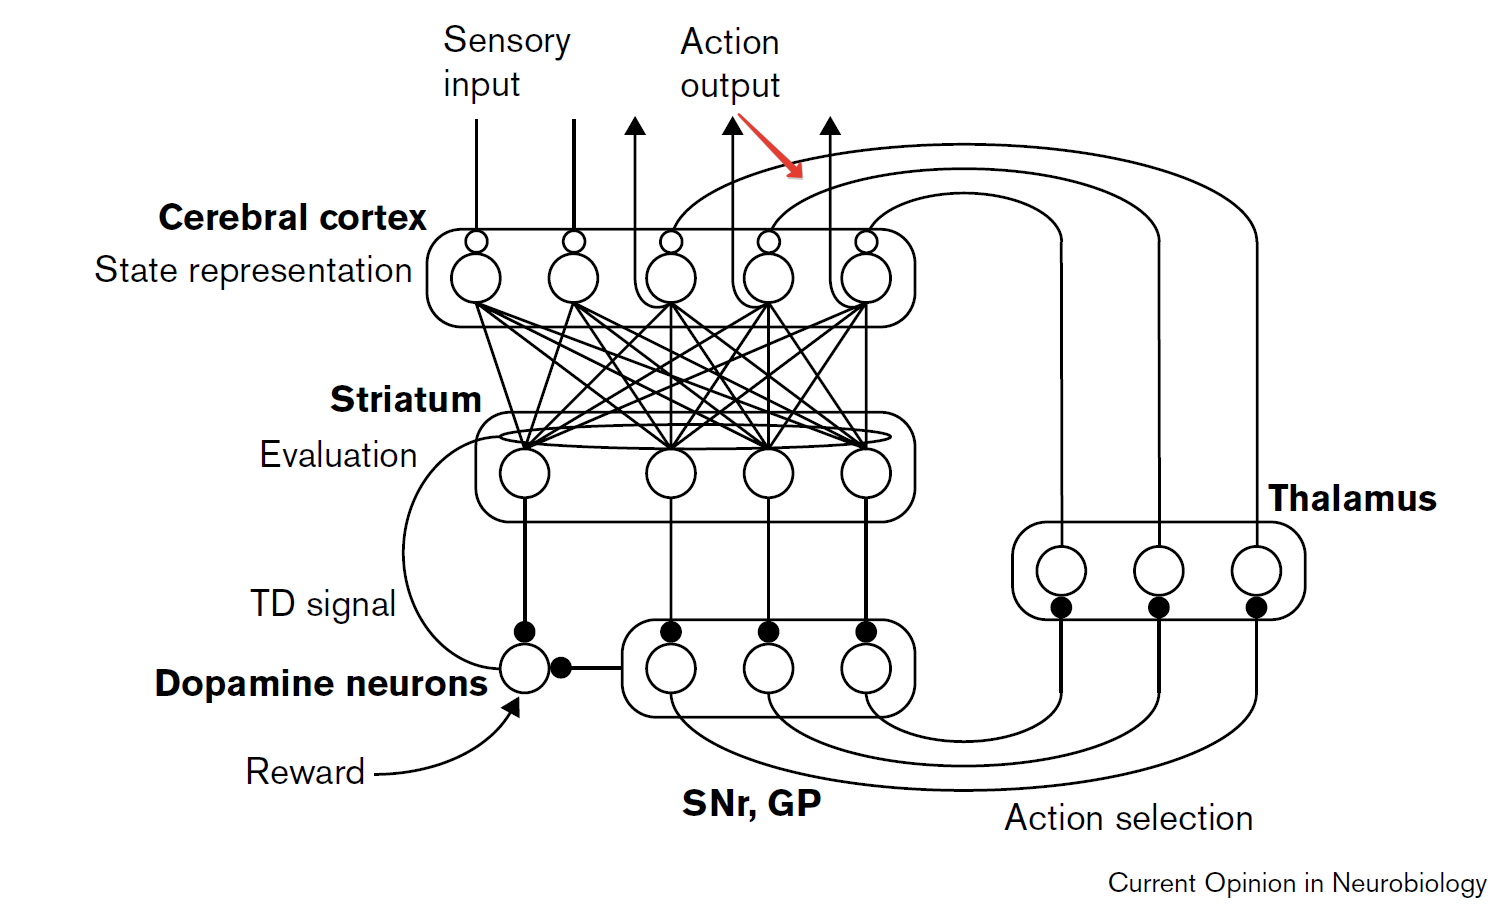
\includegraphics[width=0.8\textwidth]{misc/phisio/doya_cortico-bg}
		\caption{Цикл, образуемый корой и базальными ганглиями и реализующий обучение с подкреплением (взято из \cite{Doya2000a})}
		\label{fig:doy_cortbga}		
	\end{figure}

	Базальные ядра оценивают действия на различных уровнях сенсорно-моторной параллельной иерархии (см. \ref{fig:shumsky_schemas}). Таким образом, две иерархии: восходящая (распознавание ситуации) и нисходящая (выработка поведения) - взаимоувязываются за счет подкорковой подсистемы базальных ядер, действующей на различных временных и пространственных масштабах.
	\begin{figure}
		\centering
		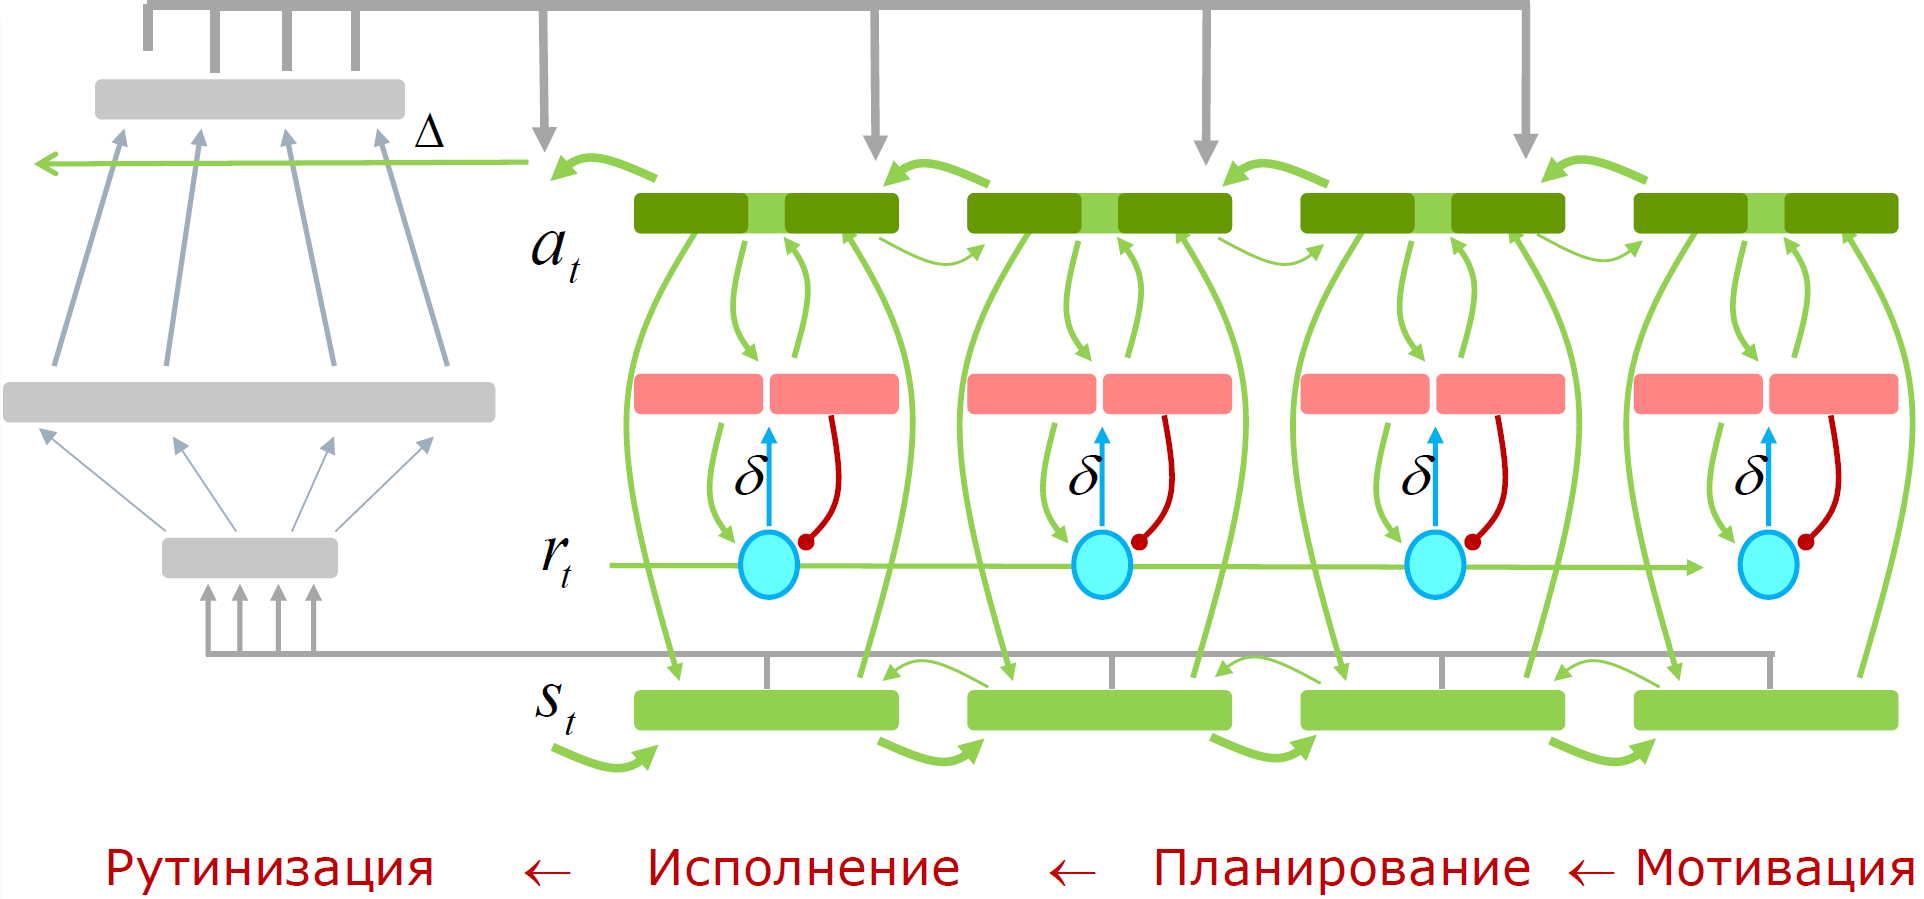
\includegraphics[width=0.8\textwidth]{misc/phisio/shumsky_schema}
		\caption{Управляющие контуры в головном мозге (обучение с учителем - мозжечок (серые участки схемы), обучение с подкреплением - базальные ганглии (средние участки схемы), обучение без учителя - кора (зеленые участки схемы)) (взято из \cite{Shumsky2015b})}
		\label{fig:shumsky_schemas}		
	\end{figure}

	Наконец, третья подсистема мозга, представленная на рис. \ref{fig:doya_schema} - мозжечок, задача которого заключается в том, чтобы, обучаясь на выработанных корой и базальными ядрами ответах на стимулы, быстро реализовывать простые решения без обратных связей и длительного поиска альтернативных путей \cite{Kawato2009}. Входными сигналами для мозжечка служат те же сигналы, что и для базальных ядер: проекции сенсорных и ассоциативных отделов коры (представление ситуаций) и, в качестве выбранного варианта действия -  проекции моторных отделов. Выходы мозжечка дополняют выходы моторных отделов коры и призваны разгрузить базально-кортикальную систему (см. рис. \ref{fig:doya_cortcer}). Мозжечок похож на обычный перцептрон, где входной сигнал поступает на большое количество гранулярных клеток ($6\cdot10^{10}$), а выход формируется большими клетками Пуркинье ($10^7$) с развитой дендритной системой ($10^5$ синапсов). Клетки Пуркинье получают сигнал от лазающего волокна, дублирующего решения коры для обучения синапсов (см. рис. \ref{fig:shumsky_schemas}).
	
	\begin{figure}
		\centering
		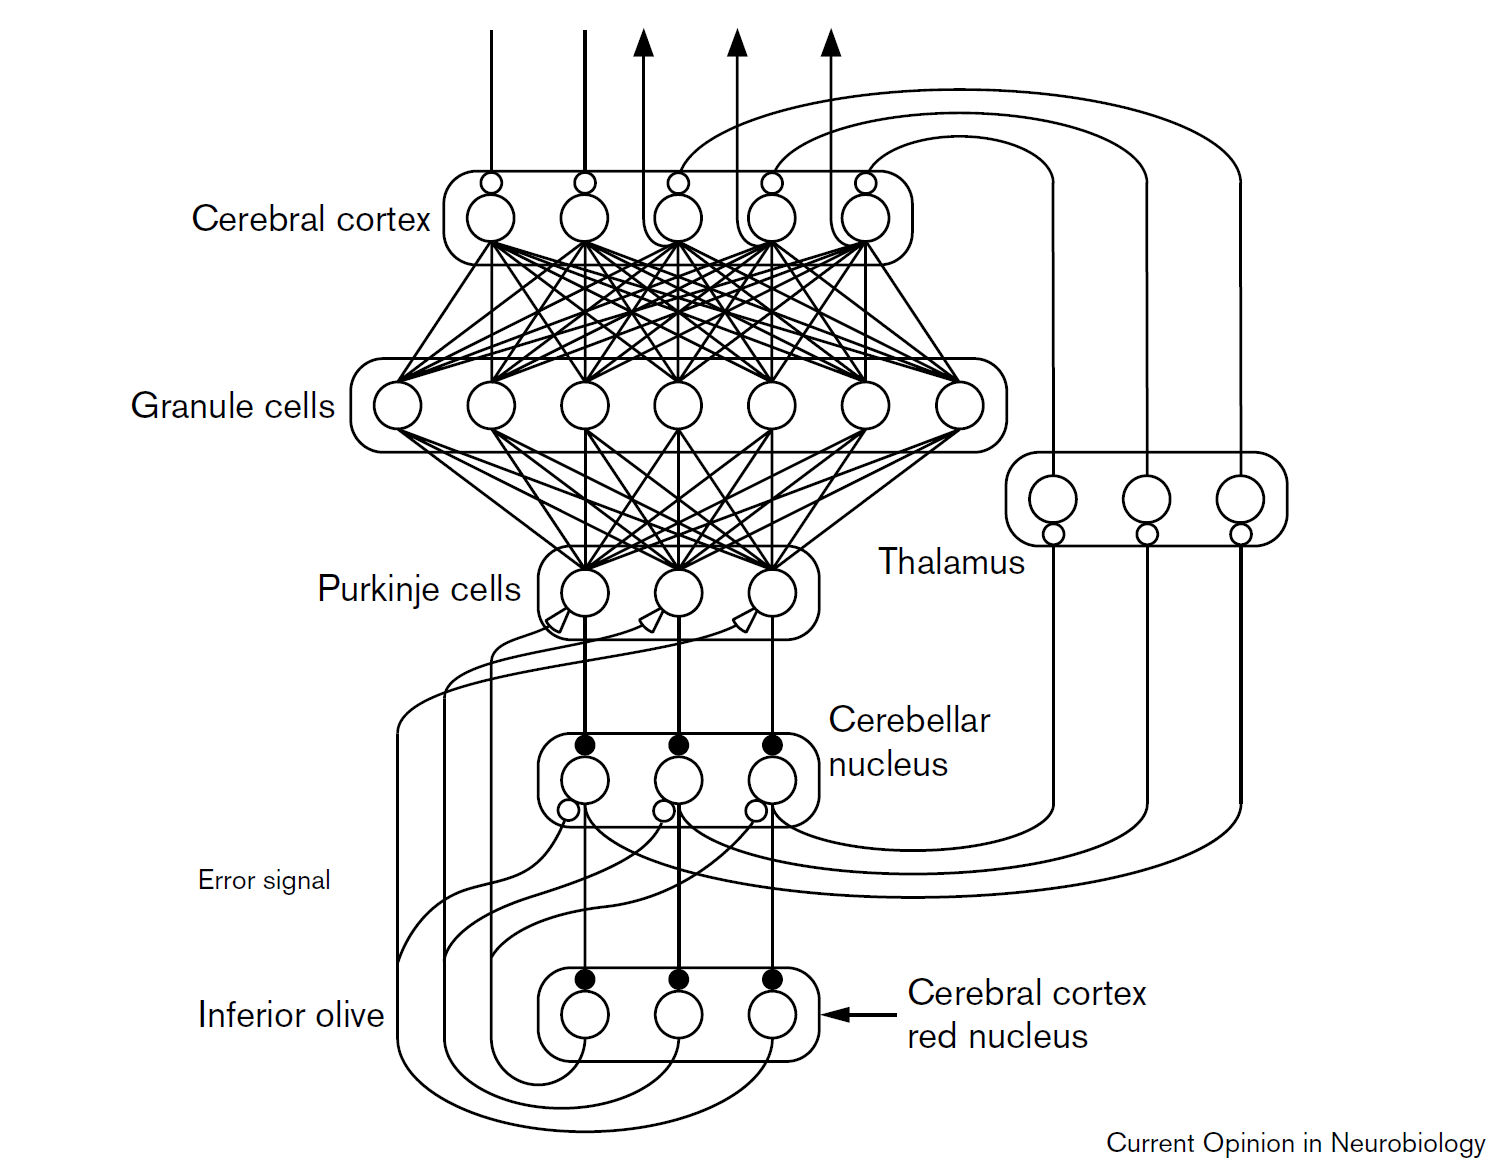
\includegraphics[width=0.7\textwidth]{misc/phisio/doya_cortico-cerebr}
		\caption{Цикл, образуемый корой и мозжечком и реализующий обучение с учителем (взято из \cite{Doya2000a})}
		\label{fig:doya_cortcer}		
	\end{figure}
	
	Некоторые общие схемы нервных цепочек изображены на рис. \ref{fig:cog_circ} и \ref{fig:cog_flow}.
	
	\begin{figure}
		\centering
		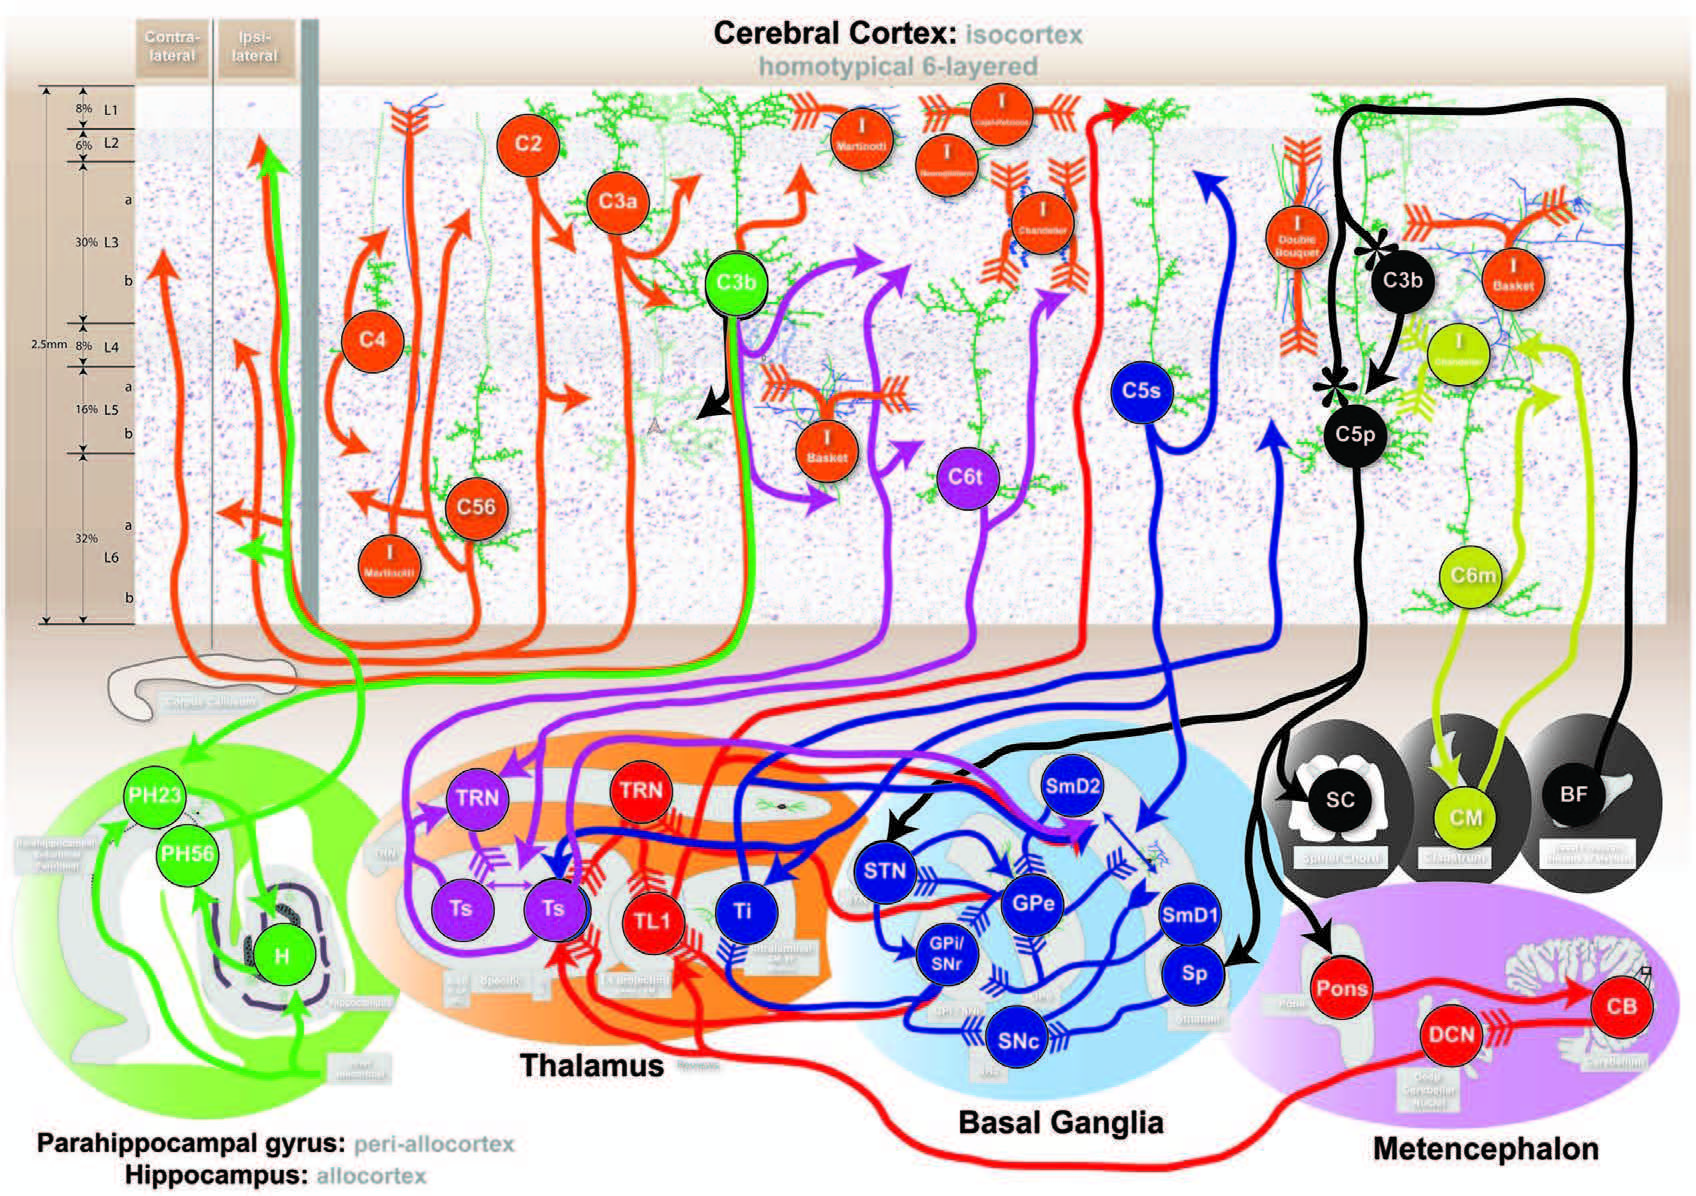
\includegraphics[width=0.8\textwidth]{misc/phisio/cognitive_circuits}
		\caption{Когнитивные цепи (взято из \cite{Solari2011}). Оранжевые стрелки - консолидация декларативной долговременной памяти, синие - выбор действий и поведенческая память, черные - реализация поведенческой памяти, красные - когнитивный контроль, желтые - регуляция потока информации в коре.}
		\label{fig:cog_circ}		
	\end{figure}

	\begin{figure}
		\centering
		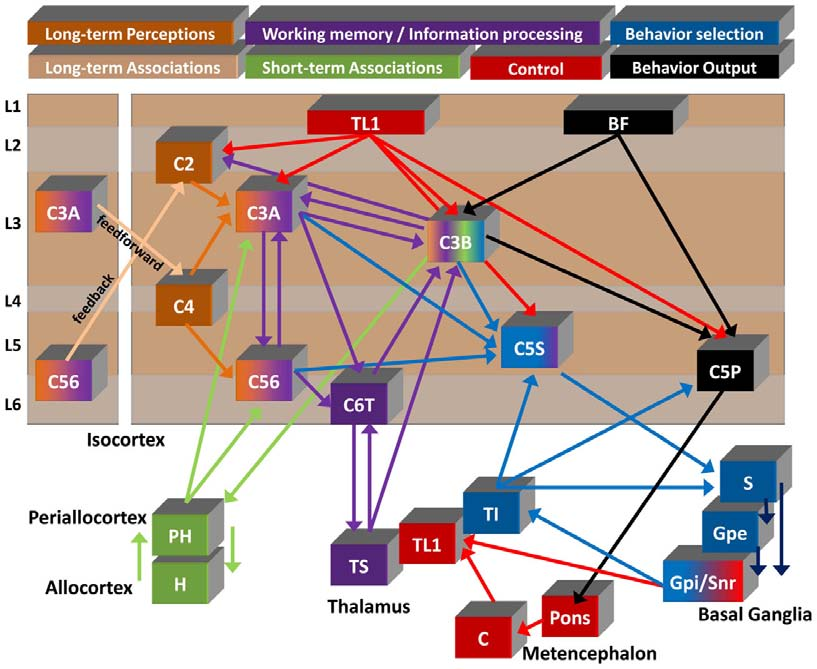
\includegraphics[width=0.8\textwidth]{misc/phisio/cognitive_flow}
		\caption{Когнитивные цепи (взято из \cite{Solari2011})}
		\label{fig:cog_flow}		
	\end{figure}

	Описанная выше схема реализовывала так называемой быстрое поведение (по Канеману \cite{Kahneman2011}). Более сложное (логическое) поведение в незнакомой ситуации вырабатывается в латеральной лобной области коры \cite{Cole2013} за счет высокой связности и синхронности работы этих отделов коры \cite{Baars2013}. Здесь происходит символьное абстрагирование от внешнего мира, что позволяет оперировать более сложными понятиями и цепочками действий не прорабатывая их в деталях. Такие, имеющие потенциальную реализацию в моторной и сенсорной иерархиях, структуры, знаки, позволяют нам мыслить без привязки к внешним сигналам в некоторой виртуальной реальности. Таким образом, знаки (или, в другой терминологии, коги \cite{Anokhin2016}) выступают вершиной некоторого сенсомоторного <<айсберга>>.

	
	\printbibliography[keyword={neuro},resetnumbers=true]
	
	\chapter{Модели картины мира}
	\section{Психосемантическая парадигма}
	
	Образ, картина мира оказывается производной от ценностно-мотивационной сферы (единичного или коллективного) субъекта познания, степени развития и характера инструментальных средств познания, от мо-дельного языка, в котором создаются образы познаваемого \cite{Petrenko2009}. Идея опосредующей роли языка в познании восходит к В. Гумбольдту, полагавшему, что <<различные языки --- не разные обозначения одного и того же предмета, а разные видения его>>, к идеям Э. Сепира - Б. Уорфа, сформулировавшим гипотезу <<лингвистической относительности>>, полагающую определяющую роль того или иного национального языка в особенностях мышления людей различных культур и в содержании их картины мира. Келли рассматривает построение картины мира обычным человеком по аналогии с ученым, создающим гипотезы о мире, проверяющим их адекватность и корректирующим их. 
	Картина мира выступает не слепком с действительности, а одной из удобных форм ее описания. <<Это карта, а не территория>>, --- пишут основатели Нейролингвистического программирования (НЛП) Р. Бэндлер	и Д. Гриндер (1995).

	Роль языка в формировании картины мира особенно высока в теории лингвистической относительности Сэпира-Уорфа: <<мы видим, слышим и воспринимаем действительность так, а не иначе в значительной мере потому, что языковые нормы нашего общества предрасполагают к определенному выбору интерпретации>>.
	
	Человек призван к сотворчеству в творении мира. Потребление без духовной работы, без решения собственных выстраданных проблем и вопросов выступает формой <<духовного онанизма>>, когда, получая примитивные <<удовольствия>>, человек дезертирует от главного предназначения --- созидания и развития своего духа, своего сознания, а через них и осуществления своего вклада в <<интегральное сознание>> (Сидерский А. Третье открытие силы. Изд. Ника-центр, 2005.).
	
	<<Большинство наших знаний о мире не были получены в нашем непосредственном личном опыте (и эмпирически не верифицируемы), а усвоены нами в школе, в общении с себе подобными, взяты из книг и художественных фильмов, из поучений родителей и средств массовой коммуникации. Не подвергаемый эмпирической проверке единичный факт тем не менее оценивается с точки зрения его правдоподобия в нашей целостной картине мира. И если вы наблюдаете вдруг появление нечто из ничего (<<чертика из табакерки>>), то вы скорее поставите под сомнение ясность своего сознания, чем на основе эмпирического опыта подвергнете сомнению закон <<сохранения вещества>>>>.
	
	<<В психологии XX века под влиянием психоанализа стали выделять область сознания и бессознательного. В философии же сохранилась более широкая трактовка понятия сознания, и когда говорят о содержании сознания, то включают туда и сознательные, и бессознательные компоненты. Понятие сознания в философской традиции оказалось близким к понятию <<картина мира>>, пришедшему из культурологи (О. Шпенглер, А.Я. Гуревич) и ставшему широко употребляемым в психологии. Понятие <<картина мира>> удобно для описания менталитета человека и общества тем, что содержит целостную структуру знания человека о мире, включающую как осознаваемые (понятийно выраженные), так и неосознаваемые и плохо осознаваемые (установки, стереотипы, психические состояния, верования и т. п.) компоненты>>
	\printbibliography[keyword={psycho},resetnumbers=true]
	
\end{document}